\documentclass[1p]{elsarticle_modified}
%\bibliographystyle{elsarticle-num}

%\usepackage[colorlinks]{hyperref}
%\usepackage{abbrmath_seonhwa} %\Abb, \Ascr, \Acal ,\Abf, \Afrak
\usepackage{amsfonts}
\usepackage{amssymb}
\usepackage{amsmath}
\usepackage{amsthm}
\usepackage{scalefnt}
\usepackage{amsbsy}
\usepackage{kotex}
\usepackage{caption}
\usepackage{subfig}
\usepackage{color}
\usepackage{graphicx}
\usepackage{xcolor} %% white, black, red, green, blue, cyan, magenta, yellow
\usepackage{float}
\usepackage{setspace}
\usepackage{hyperref}

\usepackage{tikz}
\usetikzlibrary{arrows}

\usepackage{multirow}
\usepackage{array} % fixed length table
\usepackage{hhline}

%%%%%%%%%%%%%%%%%%%%%
\makeatletter
\renewcommand*\env@matrix[1][\arraystretch]{%
	\edef\arraystretch{#1}%
	\hskip -\arraycolsep
	\let\@ifnextchar\new@ifnextchar
	\array{*\c@MaxMatrixCols c}}
\makeatother %https://tex.stackexchange.com/questions/14071/how-can-i-increase-the-line-spacing-in-a-matrix
%%%%%%%%%%%%%%%

\usepackage[normalem]{ulem}

\newcommand{\msout}[1]{\ifmmode\text{\sout{\ensuremath{#1}}}\else\sout{#1}\fi}
%SOURCE: \msout is \stkout macro in https://tex.stackexchange.com/questions/20609/strikeout-in-math-mode

\newcommand{\cancel}[1]{
	\ifmmode
	{\color{red}\msout{#1}}
	\else
	{\color{red}\sout{#1}}
	\fi
}

\newcommand{\add}[1]{
	{\color{blue}\uwave{#1}}
}

\newcommand{\replace}[2]{
	\ifmmode
	{\color{red}\msout{#1}}{\color{blue}\uwave{#2}}
	\else
	{\color{red}\sout{#1}}{\color{blue}\uwave{#2}}
	\fi
}

\newcommand{\Sol}{\mathcal{S}} %segment
\newcommand{\D}{D} %diagram
\newcommand{\A}{\mathcal{A}} %arc


%%%%%%%%%%%%%%%%%%%%%%%%%%%%%5 test

\def\sl{\operatorname{\textup{SL}}(2,\Cbb)}
\def\psl{\operatorname{\textup{PSL}}(2,\Cbb)}
\def\quan{\mkern 1mu \triangleright \mkern 1mu}

\theoremstyle{definition}
\newtheorem{thm}{Theorem}[section]
\newtheorem{prop}[thm]{Proposition}
\newtheorem{lem}[thm]{Lemma}
\newtheorem{ques}[thm]{Question}
\newtheorem{cor}[thm]{Corollary}
\newtheorem{defn}[thm]{Definition}
\newtheorem{exam}[thm]{Example}
\newtheorem{rmk}[thm]{Remark}
\newtheorem{alg}[thm]{Algorithm}

\newcommand{\I}{\sqrt{-1}}
\begin{document}

%\begin{frontmatter}
%
%\title{Boundary parabolic representations of knots up to 8 crossings}
%
%%% Group authors per affiliation:
%\author{Yunhi Cho} 
%\address{Department of Mathematics, University of Seoul, Seoul, Korea}
%\ead{yhcho@uos.ac.kr}
%
%
%\author{Seonhwa Kim} %\fnref{s_kim}}
%\address{Center for Geometry and Physics, Institute for Basic Science, Pohang, 37673, Korea}
%\ead{ryeona17@ibs.re.kr}
%
%\author{Hyuk Kim}
%\address{Department of Mathematical Sciences, Seoul National University, Seoul 08826, Korea}
%\ead{hyukkim@snu.ac.kr}
%
%\author{Seokbeom Yoon}
%\address{Department of Mathematical Sciences, Seoul National University, Seoul, 08826,  Korea}
%\ead{sbyoon15@snu.ac.kr}
%
%\begin{abstract}
%We find all boundary parabolic representation of knots up to 8 crossings.
%
%\end{abstract}
%\begin{keyword}
%    \MSC[2010] 57M25 
%\end{keyword}
%
%\end{frontmatter}

%\linenumbers
%\tableofcontents
%
\newcommand\colored[1]{\textcolor{white}{\rule[-0.35ex]{0.8em}{1.4ex}}\kern-0.8em\color{red} #1}%
%\newcommand\colored[1]{\textcolor{white}{ #1}\kern-2.17ex	\textcolor{white}{ #1}\kern-1.81ex	\textcolor{white}{ #1}\kern-2.15ex\color{red}#1	}

{\Large $\underline{12a_{0489}~(K12a_{0489})}$}

\setlength{\tabcolsep}{10pt}
\renewcommand{\arraystretch}{1.6}
\vspace{1cm}\begin{tabular}{m{100pt}>{\centering\arraybackslash}m{274pt}}
\multirow{5}{120pt}{
	\centering
	\includegraphics[width=112pt]{../../../GIT/diagram.site/Diagrams/png/1290_12a_0489.png}\\
\ \ \ A knot diagram\footnotemark}&
\allowdisplaybreaks
\textbf{Linearized knot diagam} \\
\cline{2-2}
 &
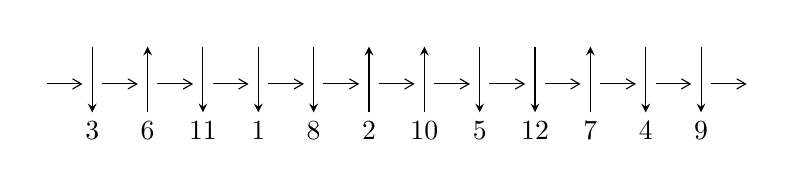
\begin{tikzpicture}[x=20pt, y=17pt]
	% nodes
	\node (C0) at (0, 0) {};
	\node (C1) at (1, 0) {};
	\node (C1U) at (1, +1) {};
	\node (C1D) at (1, -1) {3};

	\node (C2) at (2, 0) {};
	\node (C2U) at (2, +1) {};
	\node (C2D) at (2, -1) {6};

	\node (C3) at (3, 0) {};
	\node (C3U) at (3, +1) {};
	\node (C3D) at (3, -1) {11};

	\node (C4) at (4, 0) {};
	\node (C4U) at (4, +1) {};
	\node (C4D) at (4, -1) {1};

	\node (C5) at (5, 0) {};
	\node (C5U) at (5, +1) {};
	\node (C5D) at (5, -1) {8};

	\node (C6) at (6, 0) {};
	\node (C6U) at (6, +1) {};
	\node (C6D) at (6, -1) {2};

	\node (C7) at (7, 0) {};
	\node (C7U) at (7, +1) {};
	\node (C7D) at (7, -1) {10};

	\node (C8) at (8, 0) {};
	\node (C8U) at (8, +1) {};
	\node (C8D) at (8, -1) {5};

	\node (C9) at (9, 0) {};
	\node (C9U) at (9, +1) {};
	\node (C9D) at (9, -1) {12};

	\node (C10) at (10, 0) {};
	\node (C10U) at (10, +1) {};
	\node (C10D) at (10, -1) {7};

	\node (C11) at (11, 0) {};
	\node (C11U) at (11, +1) {};
	\node (C11D) at (11, -1) {4};

	\node (C12) at (12, 0) {};
	\node (C12U) at (12, +1) {};
	\node (C12D) at (12, -1) {9};
	\node (C13) at (13, 0) {};

	% arrows
	\draw[->,>={angle 60}]
	(C0) edge (C1) (C1) edge (C2) (C2) edge (C3) (C3) edge (C4) (C4) edge (C5) (C5) edge (C6) (C6) edge (C7) (C7) edge (C8) (C8) edge (C9) (C9) edge (C10) (C10) edge (C11) (C11) edge (C12) (C12) edge (C13) ;	\draw[->,>=stealth]
	(C1U) edge (C1D) (C2D) edge (C2U) (C3U) edge (C3D) (C4U) edge (C4D) (C5U) edge (C5D) (C6D) edge (C6U) (C7D) edge (C7U) (C8U) edge (C8D) (C9U) edge (C9D) (C10D) edge (C10U) (C11U) edge (C11D) (C12U) edge (C12D) ;
	\end{tikzpicture} \\
\hhline{~~} \\& 
\textbf{Solving Sequence} \\ \cline{2-2} 
 &
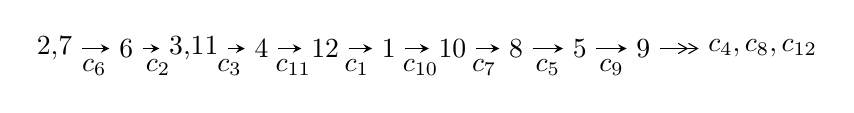
\begin{tikzpicture}[x=23pt, y=7pt]
	% node
	\node (A0) at (-1/8, 0) {2,7};
	\node (A1) at (1, 0) {6};
	\node (A2) at (33/16, 0) {3,11};
	\node (A3) at (25/8, 0) {4};
	\node (A4) at (33/8, 0) {12};
	\node (A5) at (41/8, 0) {1};
	\node (A6) at (49/8, 0) {10};
	\node (A7) at (57/8, 0) {8};
	\node (A8) at (65/8, 0) {5};
	\node (A9) at (73/8, 0) {9};
	\node (C1) at (1/2, -1) {$c_{6}$};
	\node (C2) at (3/2, -1) {$c_{2}$};
	\node (C3) at (21/8, -1) {$c_{3}$};
	\node (C4) at (29/8, -1) {$c_{11}$};
	\node (C5) at (37/8, -1) {$c_{1}$};
	\node (C6) at (45/8, -1) {$c_{10}$};
	\node (C7) at (53/8, -1) {$c_{7}$};
	\node (C8) at (61/8, -1) {$c_{5}$};
	\node (C9) at (69/8, -1) {$c_{9}$};
	\node (A10) at (11, 0) {$c_{4},c_{8},c_{12}$};

	% edge
	\draw[->,>=stealth]	
	(A0) edge (A1) (A1) edge (A2) (A2) edge (A3) (A3) edge (A4) (A4) edge (A5) (A5) edge (A6) (A6) edge (A7) (A7) edge (A8) (A8) edge (A9) ;
	\draw[->>,>={angle 60}]	
	(A9) edge (A10);
\end{tikzpicture} \\ 

\end{tabular} \\

\footnotetext{
The image of knot diagram is generated by the software ``\textbf{Draw programme}" developed by Andrew Bartholomew(\url{http://www.layer8.co.uk/maths/draw/index.htm\#Running-draw}), where we modified some parts for our purpose(\url{https://github.com/CATsTAILs/LinksPainter}).
}\phantom \\ \newline 
\centering \textbf{Ideals for irreducible components\footnotemark of $X_{\text{par}}$} 
 
\begin{align*}
I^u_{1}&=\langle 
-9.51227\times10^{329} u^{134}+5.25666\times10^{328} u^{133}+\cdots+1.45920\times10^{328} b-6.64848\times10^{331},\\
\phantom{I^u_{1}}&\phantom{= \langle  }1.39352\times10^{332} u^{134}-2.28557\times10^{332} u^{133}+\cdots+4.65486\times10^{330} a-6.26320\times10^{334},\\
\phantom{I^u_{1}}&\phantom{= \langle  }u^{135}- u^{134}+\cdots-550 u+319\rangle \\
I^u_{2}&=\langle 
-14 u^{29}-338 u^{28}+\cdots+59 b-301,\;-479 u^{29}-1526 u^{28}+\cdots+59 a+528,\;u^{30}+4 u^{29}+\cdots+u+1\rangle \\
\\
\end{align*}
\raggedright * 2 irreducible components of $\dim_{\mathbb{C}}=0$, with total 165 representations.\\
\footnotetext{All coefficients of polynomials are rational numbers. But the coefficients are sometimes approximated in decimal forms when there is not enough margin.}
\newpage
\renewcommand{\arraystretch}{1}
\centering \section*{I. $I^u_{1}= \langle -9.51\times10^{329} u^{134}+5.26\times10^{328} u^{133}+\cdots+1.46\times10^{328} b-6.65\times10^{331},\;1.39\times10^{332} u^{134}-2.29\times10^{332} u^{133}+\cdots+4.65\times10^{330} a-6.26\times10^{334},\;u^{135}- u^{134}+\cdots-550 u+319 \rangle$}
\flushleft \textbf{(i) Arc colorings}\\
\begin{tabular}{m{7pt} m{180pt} m{7pt} m{180pt} }
\flushright $a_{2}=$&$\begin{pmatrix}0\\u\end{pmatrix}$ \\
\flushright $a_{7}=$&$\begin{pmatrix}1\\0\end{pmatrix}$ \\
\flushright $a_{6}=$&$\begin{pmatrix}1\\u^2\end{pmatrix}$ \\
\flushright $a_{3}=$&$\begin{pmatrix}u\\u^3+u\end{pmatrix}$ \\
\flushright $a_{11}=$&$\begin{pmatrix}-29.9368 u^{134}+49.1008 u^{133}+\cdots-22734.0 u+13455.2\\65.1881 u^{134}-3.60242 u^{133}+\cdots+17400.5 u+4556.23\end{pmatrix}$ \\
\flushright $a_{4}=$&$\begin{pmatrix}-56.8695 u^{134}+29.8551 u^{133}+\cdots-24012.5 u+6285.24\\-7.53274 u^{134}+21.7455 u^{133}+\cdots-8585.10 u+6430.11\end{pmatrix}$ \\
\flushright $a_{12}=$&$\begin{pmatrix}-20.6048 u^{134}+99.7230 u^{133}+\cdots-31659.0 u+32778.9\\-20.8862 u^{134}-28.5899 u^{133}+\cdots+3043.27 u-12231.0\end{pmatrix}$ \\
\flushright $a_{1}=$&$\begin{pmatrix}u^3\\u^5+u^3+u\end{pmatrix}$ \\
\flushright $a_{10}=$&$\begin{pmatrix}-95.1248 u^{134}+52.7032 u^{133}+\cdots-40134.4 u+8898.94\\65.1881 u^{134}-3.60242 u^{133}+\cdots+17400.5 u+4556.23\end{pmatrix}$ \\
\flushright $a_{8}=$&$\begin{pmatrix}-66.5291 u^{134}+59.6662 u^{133}+\cdots-36144.2 u+14899.4\\48.2123 u^{134}-2.48378 u^{133}+\cdots+13350.7 u+3263.57\end{pmatrix}$ \\
\flushright $a_{5}=$&$\begin{pmatrix}-51.2429 u^{134}+2.85544 u^{133}+\cdots-14140.6 u-2321.76\\-7.95475 u^{134}+31.5932 u^{133}+\cdots-11787.9 u+9758.36\end{pmatrix}$ \\
\flushright $a_{9}=$&$\begin{pmatrix}-151.201 u^{134}+24.3816 u^{133}+\cdots-49723.1 u+1938.73\\51.2850 u^{134}+13.5590 u^{133}+\cdots+9761.08 u+8017.02\end{pmatrix}$\\&\end{tabular}
\flushleft \textbf{(ii) Obstruction class $= -1$}\\~\\
\flushleft \textbf{(iii) Cusp Shapes $= 190.854 u^{134}-52.5163 u^{133}+\cdots+60035.6 u-2114.44$}\\~\\
\newpage\renewcommand{\arraystretch}{1}
\flushleft \textbf{(iv) u-Polynomials at the component}\newline \\
\begin{tabular}{m{50pt}|m{274pt}}
Crossings & \hspace{64pt}u-Polynomials at each crossing \\
\hline $$\begin{aligned}c_{1}\end{aligned}$$&$\begin{aligned}
&u^{135}+67 u^{134}+\cdots-3424696 u-101761
\end{aligned}$\\
\hline $$\begin{aligned}c_{2},c_{6}\end{aligned}$$&$\begin{aligned}
&u^{135}- u^{134}+\cdots-550 u+319
\end{aligned}$\\
\hline $$\begin{aligned}c_{3},c_{11}\end{aligned}$$&$\begin{aligned}
&u^{135}- u^{134}+\cdots-423962 u+25289
\end{aligned}$\\
\hline $$\begin{aligned}c_{4}\end{aligned}$$&$\begin{aligned}
&u^{135}-9 u^{134}+\cdots+104857 u+98599
\end{aligned}$\\
\hline $$\begin{aligned}c_{5},c_{8}\end{aligned}$$&$\begin{aligned}
&u^{135}-6 u^{134}+\cdots+6299728 u-1729139
\end{aligned}$\\
\hline $$\begin{aligned}c_{7},c_{10}\end{aligned}$$&$\begin{aligned}
&u^{135}+6 u^{134}+\cdots+5575 u+4625
\end{aligned}$\\
\hline $$\begin{aligned}c_{9},c_{12}\end{aligned}$$&$\begin{aligned}
&u^{135}-3 u^{134}+\cdots+6999 u+481
\end{aligned}$\\
\hline
\end{tabular}\\~\\
\newpage\renewcommand{\arraystretch}{1}
\flushleft \textbf{(v) Riley Polynomials at the component}\newline \\
\begin{tabular}{m{50pt}|m{274pt}}
Crossings & \hspace{64pt}Riley Polynomials at each crossing \\
\hline $$\begin{aligned}c_{1}\end{aligned}$$&$\begin{aligned}
&y^{135}+19 y^{134}+\cdots+444067171988 y-10355301121
\end{aligned}$\\
\hline $$\begin{aligned}c_{2},c_{6}\end{aligned}$$&$\begin{aligned}
&y^{135}+67 y^{134}+\cdots-3424696 y-101761
\end{aligned}$\\
\hline $$\begin{aligned}c_{3},c_{11}\end{aligned}$$&$\begin{aligned}
&y^{135}-71 y^{134}+\cdots+117641731878 y-639533521
\end{aligned}$\\
\hline $$\begin{aligned}c_{4}\end{aligned}$$&$\begin{aligned}
&y^{135}+39 y^{134}+\cdots-1832507948977 y-9721762801
\end{aligned}$\\
\hline $$\begin{aligned}c_{5},c_{8}\end{aligned}$$&$\begin{aligned}
&y^{135}+80 y^{134}+\cdots-5136676650882 y-2989921681321
\end{aligned}$\\
\hline $$\begin{aligned}c_{7},c_{10}\end{aligned}$$&$\begin{aligned}
&y^{135}+84 y^{134}+\cdots-2837251875 y-21390625
\end{aligned}$\\
\hline $$\begin{aligned}c_{9},c_{12}\end{aligned}$$&$\begin{aligned}
&y^{135}+77 y^{134}+\cdots-2987973 y-231361
\end{aligned}$\\
\hline
\end{tabular}\\~\\
\newpage\flushleft \textbf{(vi) Complex Volumes and Cusp Shapes}
$$\begin{array}{c|c|c}  
\text{Solutions to }I^u_{1}& \I (\text{vol} + \sqrt{-1}CS) & \text{Cusp shape}\\
 \hline 
\begin{aligned}
u &= \phantom{-}0.265838 + 0.981329 I \\
a &= \phantom{-}1.17941 - 1.28721 I \\
b &= \phantom{-}1.212520 - 0.375722 I\end{aligned}
 & \phantom{-}1.78269 - 5.16544 I & \phantom{-0.000000 } 0 \\ \hline\begin{aligned}
u &= \phantom{-}0.265838 - 0.981329 I \\
a &= \phantom{-}1.17941 + 1.28721 I \\
b &= \phantom{-}1.212520 + 0.375722 I\end{aligned}
 & \phantom{-}1.78269 + 5.16544 I & \phantom{-0.000000 } 0 \\ \hline\begin{aligned}
u &= \phantom{-}0.374199 + 0.903425 I \\
a &= \phantom{-}0.722251 + 0.141191 I \\
b &= -0.48921 + 1.92440 I\end{aligned}
 & -5.05415 - 0.80188 I & \phantom{-0.000000 } 0 \\ \hline\begin{aligned}
u &= \phantom{-}0.374199 - 0.903425 I \\
a &= \phantom{-}0.722251 - 0.141191 I \\
b &= -0.48921 - 1.92440 I\end{aligned}
 & -5.05415 + 0.80188 I & \phantom{-0.000000 } 0 \\ \hline\begin{aligned}
u &= \phantom{-}0.466349 + 0.915942 I \\
a &= \phantom{-}2.36119 - 3.43185 I \\
b &= \phantom{-}0.061703 + 1.071620 I\end{aligned}
 & -0.25900 + 2.18550 I & \phantom{-0.000000 } 0 \\ \hline\begin{aligned}
u &= \phantom{-}0.466349 - 0.915942 I \\
a &= \phantom{-}2.36119 + 3.43185 I \\
b &= \phantom{-}0.061703 - 1.071620 I\end{aligned}
 & -0.25900 - 2.18550 I & \phantom{-0.000000 } 0 \\ \hline\begin{aligned}
u &= \phantom{-}0.364886 + 0.900855 I \\
a &= -1.28870 + 0.61504 I \\
b &= -0.13762 - 1.95311 I\end{aligned}
 & -5.02629 + 3.85941 I & \phantom{-0.000000 } 0 \\ \hline\begin{aligned}
u &= \phantom{-}0.364886 - 0.900855 I \\
a &= -1.28870 - 0.61504 I \\
b &= -0.13762 + 1.95311 I\end{aligned}
 & -5.02629 - 3.85941 I & \phantom{-0.000000 } 0 \\ \hline\begin{aligned}
u &= \phantom{-}0.457705 + 0.927031 I \\
a &= -0.261377 + 0.984995 I \\
b &= -0.028770 - 0.159842 I\end{aligned}
 & \phantom{-}1.65847 + 2.09523 I & \phantom{-0.000000 } 0 \\ \hline\begin{aligned}
u &= \phantom{-}0.457705 - 0.927031 I \\
a &= -0.261377 - 0.984995 I \\
b &= -0.028770 + 0.159842 I\end{aligned}
 & \phantom{-}1.65847 - 2.09523 I & \phantom{-0.000000 } 0\\
 \hline 
 \end{array}$$\newpage$$\begin{array}{c|c|c}  
\text{Solutions to }I^u_{1}& \I (\text{vol} + \sqrt{-1}CS) & \text{Cusp shape}\\
 \hline 
\begin{aligned}
u &= \phantom{-}0.726714 + 0.633434 I \\
a &= \phantom{-}0.05426 + 1.55018 I \\
b &= -0.461684 + 1.097510 I\end{aligned}
 & -2.12663 - 0.80068 I & \phantom{-0.000000 } 0 \\ \hline\begin{aligned}
u &= \phantom{-}0.726714 - 0.633434 I \\
a &= \phantom{-}0.05426 - 1.55018 I \\
b &= -0.461684 - 1.097510 I\end{aligned}
 & -2.12663 + 0.80068 I & \phantom{-0.000000 } 0 \\ \hline\begin{aligned}
u &= -0.187369 + 0.943857 I \\
a &= -1.63419 - 1.84417 I \\
b &= \phantom{-}0.222091 + 0.743291 I\end{aligned}
 & \phantom{-}2.09254 + 5.74840 I & \phantom{-0.000000 } 0 \\ \hline\begin{aligned}
u &= -0.187369 - 0.943857 I \\
a &= -1.63419 + 1.84417 I \\
b &= \phantom{-}0.222091 - 0.743291 I\end{aligned}
 & \phantom{-}2.09254 - 5.74840 I & \phantom{-0.000000 } 0 \\ \hline\begin{aligned}
u &= -0.215758 + 0.932206 I \\
a &= \phantom{-}1.64183 + 1.13518 I \\
b &= \phantom{-}0.086520 - 0.953014 I\end{aligned}
 & -2.76081 + 1.33759 I & \phantom{-0.000000 } 0 \\ \hline\begin{aligned}
u &= -0.215758 - 0.932206 I \\
a &= \phantom{-}1.64183 - 1.13518 I \\
b &= \phantom{-}0.086520 + 0.953014 I\end{aligned}
 & -2.76081 - 1.33759 I & \phantom{-0.000000 } 0 \\ \hline\begin{aligned}
u &= -0.767637 + 0.717888 I \\
a &= \phantom{-}1.206440 + 0.058732 I \\
b &= \phantom{-}0.927206 - 0.460326 I\end{aligned}
 & \phantom{-}8.78928 + 1.19131 I & \phantom{-0.000000 } 0 \\ \hline\begin{aligned}
u &= -0.767637 - 0.717888 I \\
a &= \phantom{-}1.206440 - 0.058732 I \\
b &= \phantom{-}0.927206 + 0.460326 I\end{aligned}
 & \phantom{-}8.78928 - 1.19131 I & \phantom{-0.000000 } 0 \\ \hline\begin{aligned}
u &= -0.845569 + 0.417929 I \\
a &= -0.717754 - 1.122110 I \\
b &= -0.379717 - 1.235620 I\end{aligned}
 & -2.20552 + 7.02826 I & \phantom{-0.000000 } 0 \\ \hline\begin{aligned}
u &= -0.845569 - 0.417929 I \\
a &= -0.717754 + 1.122110 I \\
b &= -0.379717 + 1.235620 I\end{aligned}
 & -2.20552 - 7.02826 I & \phantom{-0.000000 } 0\\
 \hline 
 \end{array}$$\newpage$$\begin{array}{c|c|c}  
\text{Solutions to }I^u_{1}& \I (\text{vol} + \sqrt{-1}CS) & \text{Cusp shape}\\
 \hline 
\begin{aligned}
u &= -0.882693 + 0.331756 I \\
a &= \phantom{-}0.676897 + 0.927144 I \\
b &= \phantom{-}0.281110 + 1.065570 I\end{aligned}
 & -4.24619 + 2.41039 I & \phantom{-0.000000 } 0 \\ \hline\begin{aligned}
u &= -0.882693 - 0.331756 I \\
a &= \phantom{-}0.676897 - 0.927144 I \\
b &= \phantom{-}0.281110 - 1.065570 I\end{aligned}
 & -4.24619 - 2.41039 I & \phantom{-0.000000 } 0 \\ \hline\begin{aligned}
u &= \phantom{-}0.994252 + 0.374540 I \\
a &= \phantom{-}0.744033 - 0.927671 I \\
b &= \phantom{-}0.68805 - 1.26056 I\end{aligned}
 & \phantom{-}3.02874 - 13.26000 I & \phantom{-0.000000 } 0 \\ \hline\begin{aligned}
u &= \phantom{-}0.994252 - 0.374540 I \\
a &= \phantom{-}0.744033 + 0.927671 I \\
b &= \phantom{-}0.68805 + 1.26056 I\end{aligned}
 & \phantom{-}3.02874 + 13.26000 I & \phantom{-0.000000 } 0 \\ \hline\begin{aligned}
u &= -0.371813 + 0.995584 I \\
a &= -0.385802 - 0.791456 I \\
b &= -0.989393 - 0.610559 I\end{aligned}
 & -1.062960 + 0.685920 I & \phantom{-0.000000 } 0 \\ \hline\begin{aligned}
u &= -0.371813 - 0.995584 I \\
a &= -0.385802 + 0.791456 I \\
b &= -0.989393 + 0.610559 I\end{aligned}
 & -1.062960 - 0.685920 I & \phantom{-0.000000 } 0 \\ \hline\begin{aligned}
u &= \phantom{-}0.760598 + 0.544727 I \\
a &= -1.147330 + 0.724272 I \\
b &= -0.892174 - 0.333012 I\end{aligned}
 & \phantom{-}1.94041 - 1.29727 I & \phantom{-0.000000 } 0 \\ \hline\begin{aligned}
u &= \phantom{-}0.760598 - 0.544727 I \\
a &= -1.147330 - 0.724272 I \\
b &= -0.892174 + 0.333012 I\end{aligned}
 & \phantom{-}1.94041 + 1.29727 I & \phantom{-0.000000 } 0 \\ \hline\begin{aligned}
u &= \phantom{-}0.286519 + 0.890166 I \\
a &= -1.144710 + 0.645186 I \\
b &= -0.776901 + 0.765914 I\end{aligned}
 & -2.15556 - 0.91680 I & \phantom{-0.000000 } 0 \\ \hline\begin{aligned}
u &= \phantom{-}0.286519 - 0.890166 I \\
a &= -1.144710 - 0.645186 I \\
b &= -0.776901 - 0.765914 I\end{aligned}
 & -2.15556 + 0.91680 I & \phantom{-0.000000 } 0\\
 \hline 
 \end{array}$$\newpage$$\begin{array}{c|c|c}  
\text{Solutions to }I^u_{1}& \I (\text{vol} + \sqrt{-1}CS) & \text{Cusp shape}\\
 \hline 
\begin{aligned}
u &= -0.777318 + 0.518275 I \\
a &= -0.227730 - 0.343635 I \\
b &= -0.510637 - 1.102750 I\end{aligned}
 & \phantom{-}1.74694 + 2.14723 I & \phantom{-0.000000 } 0 \\ \hline\begin{aligned}
u &= -0.777318 - 0.518275 I \\
a &= -0.227730 + 0.343635 I \\
b &= -0.510637 + 1.102750 I\end{aligned}
 & \phantom{-}1.74694 - 2.14723 I & \phantom{-0.000000 } 0 \\ \hline\begin{aligned}
u &= \phantom{-}0.383945 + 0.995155 I \\
a &= -1.24783 + 1.35174 I \\
b &= -0.399140 - 1.173020 I\end{aligned}
 & -2.82130 + 3.53514 I & \phantom{-0.000000 } 0 \\ \hline\begin{aligned}
u &= \phantom{-}0.383945 - 0.995155 I \\
a &= -1.24783 - 1.35174 I \\
b &= -0.399140 + 1.173020 I\end{aligned}
 & -2.82130 - 3.53514 I & \phantom{-0.000000 } 0 \\ \hline\begin{aligned}
u &= \phantom{-}0.762367 + 0.536952 I \\
a &= -0.225190 - 1.365020 I \\
b &= \phantom{-}0.100144 - 1.238080 I\end{aligned}
 & -1.39518 + 3.66830 I & \phantom{-0.000000 } 0 \\ \hline\begin{aligned}
u &= \phantom{-}0.762367 - 0.536952 I \\
a &= -0.225190 + 1.365020 I \\
b &= \phantom{-}0.100144 + 1.238080 I\end{aligned}
 & -1.39518 - 3.66830 I & \phantom{-0.000000 } 0 \\ \hline\begin{aligned}
u &= \phantom{-}0.825777 + 0.425793 I \\
a &= \phantom{-}1.160950 + 0.112814 I \\
b &= \phantom{-}0.757772 + 0.811822 I\end{aligned}
 & \phantom{-}6.25152 + 3.96870 I & \phantom{-0.000000 } 0 \\ \hline\begin{aligned}
u &= \phantom{-}0.825777 - 0.425793 I \\
a &= \phantom{-}1.160950 - 0.112814 I \\
b &= \phantom{-}0.757772 - 0.811822 I\end{aligned}
 & \phantom{-}6.25152 - 3.96870 I & \phantom{-0.000000 } 0 \\ \hline\begin{aligned}
u &= -0.339820 + 0.847663 I \\
a &= -1.88123 - 0.73761 I \\
b &= -0.689407 + 1.031730 I\end{aligned}
 & -0.57479 - 3.50977 I & \phantom{-0.000000 } 0 \\ \hline\begin{aligned}
u &= -0.339820 - 0.847663 I \\
a &= -1.88123 + 0.73761 I \\
b &= -0.689407 - 1.031730 I\end{aligned}
 & -0.57479 + 3.50977 I & \phantom{-0.000000 } 0\\
 \hline 
 \end{array}$$\newpage$$\begin{array}{c|c|c}  
\text{Solutions to }I^u_{1}& \I (\text{vol} + \sqrt{-1}CS) & \text{Cusp shape}\\
 \hline 
\begin{aligned}
u &= \phantom{-}0.551339 + 0.944571 I \\
a &= -2.80537 - 0.87573 I \\
b &= -0.120919 - 0.877859 I\end{aligned}
 & \phantom{-}0.33137 + 2.46359 I & \phantom{-0.000000 } 0 \\ \hline\begin{aligned}
u &= \phantom{-}0.551339 - 0.944571 I \\
a &= -2.80537 + 0.87573 I \\
b &= -0.120919 + 0.877859 I\end{aligned}
 & \phantom{-}0.33137 - 2.46359 I & \phantom{-0.000000 } 0 \\ \hline\begin{aligned}
u &= -0.747098 + 0.496691 I \\
a &= \phantom{-}0.753327 + 0.338635 I \\
b &= \phantom{-}0.643260 + 1.114100 I\end{aligned}
 & \phantom{-}6.73489 + 6.90205 I & \phantom{-0.000000 } 0 \\ \hline\begin{aligned}
u &= -0.747098 - 0.496691 I \\
a &= \phantom{-}0.753327 - 0.338635 I \\
b &= \phantom{-}0.643260 - 1.114100 I\end{aligned}
 & \phantom{-}6.73489 - 6.90205 I & \phantom{-0.000000 } 0 \\ \hline\begin{aligned}
u &= \phantom{-}1.055650 + 0.320503 I \\
a &= -0.596178 + 0.716528 I \\
b &= -0.576598 + 1.162180 I\end{aligned}
 & -0.57907 - 6.64964 I & \phantom{-0.000000 } 0 \\ \hline\begin{aligned}
u &= \phantom{-}1.055650 - 0.320503 I \\
a &= -0.596178 - 0.716528 I \\
b &= -0.576598 - 1.162180 I\end{aligned}
 & -0.57907 + 6.64964 I & \phantom{-0.000000 } 0 \\ \hline\begin{aligned}
u &= \phantom{-}0.582769 + 0.680195 I \\
a &= -0.10177 + 1.82737 I \\
b &= \phantom{-}0.139332 + 0.691801 I\end{aligned}
 & \phantom{-}1.10381 + 2.08367 I & \phantom{-0.000000 } 0 \\ \hline\begin{aligned}
u &= \phantom{-}0.582769 - 0.680195 I \\
a &= -0.10177 - 1.82737 I \\
b &= \phantom{-}0.139332 - 0.691801 I\end{aligned}
 & \phantom{-}1.10381 - 2.08367 I & \phantom{-0.000000 } 0 \\ \hline\begin{aligned}
u &= -0.720243 + 0.838281 I \\
a &= -0.867162 - 0.508026 I \\
b &= -0.894294 + 0.127528 I\end{aligned}
 & \phantom{-}4.68723 - 2.72448 I & \phantom{-0.000000 } 0 \\ \hline\begin{aligned}
u &= -0.720243 - 0.838281 I \\
a &= -0.867162 + 0.508026 I \\
b &= -0.894294 - 0.127528 I\end{aligned}
 & \phantom{-}4.68723 + 2.72448 I & \phantom{-0.000000 } 0\\
 \hline 
 \end{array}$$\newpage$$\begin{array}{c|c|c}  
\text{Solutions to }I^u_{1}& \I (\text{vol} + \sqrt{-1}CS) & \text{Cusp shape}\\
 \hline 
\begin{aligned}
u &= -0.794872 + 0.399127 I \\
a &= \phantom{-}0.036138 - 0.214370 I \\
b &= \phantom{-}0.480545 + 0.887485 I\end{aligned}
 & \phantom{-}5.21269 - 4.11478 I & \phantom{-0.000000 } 0 \\ \hline\begin{aligned}
u &= -0.794872 - 0.399127 I \\
a &= \phantom{-}0.036138 + 0.214370 I \\
b &= \phantom{-}0.480545 - 0.887485 I\end{aligned}
 & \phantom{-}5.21269 + 4.11478 I & \phantom{-0.000000 } 0 \\ \hline\begin{aligned}
u &= \phantom{-}0.435199 + 0.764743 I \\
a &= \phantom{-}2.23715 - 0.91291 I \\
b &= \phantom{-}0.094622 - 0.861347 I\end{aligned}
 & \phantom{-}0.22529 + 1.62225 I & \phantom{-0.000000 } 0 \\ \hline\begin{aligned}
u &= \phantom{-}0.435199 - 0.764743 I \\
a &= \phantom{-}2.23715 + 0.91291 I \\
b &= \phantom{-}0.094622 + 0.861347 I\end{aligned}
 & \phantom{-}0.22529 - 1.62225 I & \phantom{-0.000000 } 0 \\ \hline\begin{aligned}
u &= \phantom{-}0.854569 + 0.205012 I \\
a &= \phantom{-}0.877909 - 0.294115 I \\
b &= \phantom{-}0.681772 - 0.870366 I\end{aligned}
 & \phantom{-}6.02008 - 1.50841 I & \phantom{-0.000000 } 0 \\ \hline\begin{aligned}
u &= \phantom{-}0.854569 - 0.205012 I \\
a &= \phantom{-}0.877909 + 0.294115 I \\
b &= \phantom{-}0.681772 + 0.870366 I\end{aligned}
 & \phantom{-}6.02008 + 1.50841 I & \phantom{-0.000000 } 0 \\ \hline\begin{aligned}
u &= \phantom{-}0.283631 + 1.099650 I \\
a &= \phantom{-}1.05280 - 1.40620 I \\
b &= \phantom{-}0.754219 + 0.915733 I\end{aligned}
 & \phantom{-}1.46017 + 6.59736 I & \phantom{-0.000000 } 0 \\ \hline\begin{aligned}
u &= \phantom{-}0.283631 - 1.099650 I \\
a &= \phantom{-}1.05280 + 1.40620 I \\
b &= \phantom{-}0.754219 - 0.915733 I\end{aligned}
 & \phantom{-}1.46017 - 6.59736 I & \phantom{-0.000000 } 0 \\ \hline\begin{aligned}
u &= -0.290029 + 1.099260 I \\
a &= \phantom{-}0.857895 + 0.027587 I \\
b &= -0.35741 - 1.62292 I\end{aligned}
 & -4.65362 - 0.62051 I & \phantom{-0.000000 } 0 \\ \hline\begin{aligned}
u &= -0.290029 - 1.099260 I \\
a &= \phantom{-}0.857895 - 0.027587 I \\
b &= -0.35741 + 1.62292 I\end{aligned}
 & -4.65362 + 0.62051 I & \phantom{-0.000000 } 0\\
 \hline 
 \end{array}$$\newpage$$\begin{array}{c|c|c}  
\text{Solutions to }I^u_{1}& \I (\text{vol} + \sqrt{-1}CS) & \text{Cusp shape}\\
 \hline 
\begin{aligned}
u &= -0.421078 + 1.060170 I \\
a &= \phantom{-}0.834382 + 0.516928 I \\
b &= \phantom{-}0.708648 + 0.317851 I\end{aligned}
 & -4.23295 - 3.45370 I & \phantom{-0.000000 } 0 \\ \hline\begin{aligned}
u &= -0.421078 - 1.060170 I \\
a &= \phantom{-}0.834382 - 0.516928 I \\
b &= \phantom{-}0.708648 - 0.317851 I\end{aligned}
 & -4.23295 + 3.45370 I & \phantom{-0.000000 } 0 \\ \hline\begin{aligned}
u &= \phantom{-}0.328998 + 1.094430 I \\
a &= -0.444577 + 0.507036 I \\
b &= \phantom{-}0.378405 - 0.621872 I\end{aligned}
 & \phantom{-}1.84843 + 2.01030 I & \phantom{-0.000000 } 0 \\ \hline\begin{aligned}
u &= \phantom{-}0.328998 - 1.094430 I \\
a &= -0.444577 - 0.507036 I \\
b &= \phantom{-}0.378405 + 0.621872 I\end{aligned}
 & \phantom{-}1.84843 - 2.01030 I & \phantom{-0.000000 } 0 \\ \hline\begin{aligned}
u &= \phantom{-}0.699652 + 0.486084 I \\
a &= \phantom{-}1.76471 - 0.81801 I \\
b &= \phantom{-}1.224430 + 0.443019 I\end{aligned}
 & \phantom{-}5.79170 - 6.57634 I & \phantom{-0.000000 } 0 \\ \hline\begin{aligned}
u &= \phantom{-}0.699652 - 0.486084 I \\
a &= \phantom{-}1.76471 + 0.81801 I \\
b &= \phantom{-}1.224430 - 0.443019 I\end{aligned}
 & \phantom{-}5.79170 + 6.57634 I & \phantom{-0.000000 } 0 \\ \hline\begin{aligned}
u &= \phantom{-}0.504710 + 1.034030 I \\
a &= \phantom{-}1.53961 - 0.41211 I \\
b &= \phantom{-}0.141439 + 1.014040 I\end{aligned}
 & -1.94154 + 2.70157 I & \phantom{-0.000000 } 0 \\ \hline\begin{aligned}
u &= \phantom{-}0.504710 - 1.034030 I \\
a &= \phantom{-}1.53961 + 0.41211 I \\
b &= \phantom{-}0.141439 - 1.014040 I\end{aligned}
 & -1.94154 - 2.70157 I & \phantom{-0.000000 } 0 \\ \hline\begin{aligned}
u &= -0.288709 + 1.116640 I \\
a &= -0.549556 + 0.260093 I \\
b &= \phantom{-}0.67576 + 1.51289 I\end{aligned}
 & -4.62033 + 0.51627 I & \phantom{-0.000000 } 0 \\ \hline\begin{aligned}
u &= -0.288709 - 1.116640 I \\
a &= -0.549556 - 0.260093 I \\
b &= \phantom{-}0.67576 - 1.51289 I\end{aligned}
 & -4.62033 - 0.51627 I & \phantom{-0.000000 } 0\\
 \hline 
 \end{array}$$\newpage$$\begin{array}{c|c|c}  
\text{Solutions to }I^u_{1}& \I (\text{vol} + \sqrt{-1}CS) & \text{Cusp shape}\\
 \hline 
\begin{aligned}
u &= \phantom{-}0.601897 + 1.005360 I \\
a &= -1.83629 - 0.18029 I \\
b &= -0.77300 - 1.30337 I\end{aligned}
 & -3.27840 + 5.88202 I & \phantom{-0.000000 } 0 \\ \hline\begin{aligned}
u &= \phantom{-}0.601897 - 1.005360 I \\
a &= -1.83629 + 0.18029 I \\
b &= -0.77300 + 1.30337 I\end{aligned}
 & -3.27840 - 5.88202 I & \phantom{-0.000000 } 0 \\ \hline\begin{aligned}
u &= -0.493673 + 1.079570 I \\
a &= -1.20529 - 0.83975 I \\
b &= -0.985626 + 0.155345 I\end{aligned}
 & -0.09723 - 7.30650 I & \phantom{-0.000000 } 0 \\ \hline\begin{aligned}
u &= -0.493673 - 1.079570 I \\
a &= -1.20529 + 0.83975 I \\
b &= -0.985626 - 0.155345 I\end{aligned}
 & -0.09723 + 7.30650 I & \phantom{-0.000000 } 0 \\ \hline\begin{aligned}
u &= -0.725373 + 0.950534 I \\
a &= \phantom{-}0.447350 + 0.864511 I \\
b &= \phantom{-}0.874319 + 0.296644 I\end{aligned}
 & \phantom{-}8.11492 - 6.80194 I & \phantom{-0.000000 } 0 \\ \hline\begin{aligned}
u &= -0.725373 - 0.950534 I \\
a &= \phantom{-}0.447350 - 0.864511 I \\
b &= \phantom{-}0.874319 - 0.296644 I\end{aligned}
 & \phantom{-}8.11492 + 6.80194 I & \phantom{-0.000000 } 0 \\ \hline\begin{aligned}
u &= -0.126354 + 1.191560 I \\
a &= \phantom{-}0.061222 + 0.642052 I \\
b &= -0.22556 - 1.43840 I\end{aligned}
 & -7.70180 + 4.47507 I & \phantom{-0.000000 } 0 \\ \hline\begin{aligned}
u &= -0.126354 - 1.191560 I \\
a &= \phantom{-}0.061222 - 0.642052 I \\
b &= -0.22556 + 1.43840 I\end{aligned}
 & -7.70180 - 4.47507 I & \phantom{-0.000000 } 0 \\ \hline\begin{aligned}
u &= \phantom{-}0.599444 + 1.045410 I \\
a &= \phantom{-}1.64387 + 0.31409 I \\
b &= \phantom{-}0.32716 + 1.42597 I\end{aligned}
 & -2.94318 + 1.48770 I & \phantom{-0.000000 } 0 \\ \hline\begin{aligned}
u &= \phantom{-}0.599444 - 1.045410 I \\
a &= \phantom{-}1.64387 - 0.31409 I \\
b &= \phantom{-}0.32716 - 1.42597 I\end{aligned}
 & -2.94318 - 1.48770 I & \phantom{-0.000000 } 0\\
 \hline 
 \end{array}$$\newpage$$\begin{array}{c|c|c}  
\text{Solutions to }I^u_{1}& \I (\text{vol} + \sqrt{-1}CS) & \text{Cusp shape}\\
 \hline 
\begin{aligned}
u &= \phantom{-}0.610787 + 1.044940 I \\
a &= -0.865488 + 0.496487 I \\
b &= -1.171840 + 0.081867 I\end{aligned}
 & \phantom{-}0.42795 + 6.48627 I & \phantom{-0.000000 } 0 \\ \hline\begin{aligned}
u &= \phantom{-}0.610787 - 1.044940 I \\
a &= -0.865488 - 0.496487 I \\
b &= -1.171840 - 0.081867 I\end{aligned}
 & \phantom{-}0.42795 - 6.48627 I & \phantom{-0.000000 } 0 \\ \hline\begin{aligned}
u &= \phantom{-}0.583969 + 1.063090 I \\
a &= \phantom{-}0.817273 - 0.921378 I \\
b &= \phantom{-}1.52568 - 0.31930 I\end{aligned}
 & \phantom{-}4.07484 + 11.53030 I & \phantom{-0.000000 } 0 \\ \hline\begin{aligned}
u &= \phantom{-}0.583969 - 1.063090 I \\
a &= \phantom{-}0.817273 + 0.921378 I \\
b &= \phantom{-}1.52568 + 0.31930 I\end{aligned}
 & \phantom{-}4.07484 - 11.53030 I & \phantom{-0.000000 } 0 \\ \hline\begin{aligned}
u &= -0.337676 + 1.175430 I \\
a &= -1.38803 - 0.92224 I \\
b &= -0.087836 + 0.410444 I\end{aligned}
 & \phantom{-}0.58386 - 7.10567 I & \phantom{-0.000000 } 0 \\ \hline\begin{aligned}
u &= -0.337676 - 1.175430 I \\
a &= -1.38803 + 0.92224 I \\
b &= -0.087836 - 0.410444 I\end{aligned}
 & \phantom{-}0.58386 + 7.10567 I & \phantom{-0.000000 } 0 \\ \hline\begin{aligned}
u &= -0.613282 + 1.062090 I \\
a &= -1.34536 - 0.61312 I \\
b &= -0.418964 + 1.329760 I\end{aligned}
 & \phantom{-}0.10371 - 7.38645 I & \phantom{-0.000000 } 0 \\ \hline\begin{aligned}
u &= -0.613282 - 1.062090 I \\
a &= -1.34536 + 0.61312 I \\
b &= -0.418964 - 1.329760 I\end{aligned}
 & \phantom{-}0.10371 + 7.38645 I & \phantom{-0.000000 } 0 \\ \hline\begin{aligned}
u &= -0.606712 + 1.066770 I \\
a &= \phantom{-}1.58179 + 0.92970 I \\
b &= \phantom{-}0.539517 - 1.251280 I\end{aligned}
 & \phantom{-}5.03139 - 12.05540 I & \phantom{-0.000000 } 0 \\ \hline\begin{aligned}
u &= -0.606712 - 1.066770 I \\
a &= \phantom{-}1.58179 - 0.92970 I \\
b &= \phantom{-}0.539517 + 1.251280 I\end{aligned}
 & \phantom{-}5.03139 + 12.05540 I & \phantom{-0.000000 } 0\\
 \hline 
 \end{array}$$\newpage$$\begin{array}{c|c|c}  
\text{Solutions to }I^u_{1}& \I (\text{vol} + \sqrt{-1}CS) & \text{Cusp shape}\\
 \hline 
\begin{aligned}
u &= -0.549921 + 1.102620 I \\
a &= -1.83190 - 0.45737 I \\
b &= -0.88035 + 1.41293 I\end{aligned}
 & -2.89414 - 6.77157 I & \phantom{-0.000000 } 0 \\ \hline\begin{aligned}
u &= -0.549921 - 1.102620 I \\
a &= -1.83190 + 0.45737 I \\
b &= -0.88035 - 1.41293 I\end{aligned}
 & -2.89414 + 6.77157 I & \phantom{-0.000000 } 0 \\ \hline\begin{aligned}
u &= -0.709740 + 0.288840 I \\
a &= \phantom{-}1.34883 + 1.51456 I \\
b &= \phantom{-}0.901939 + 1.056320 I\end{aligned}
 & -0.51947 + 3.40508 I & \phantom{-0.000000 } 0 \\ \hline\begin{aligned}
u &= -0.709740 - 0.288840 I \\
a &= \phantom{-}1.34883 - 1.51456 I \\
b &= \phantom{-}0.901939 - 1.056320 I\end{aligned}
 & -0.51947 - 3.40508 I & \phantom{-0.000000 } 0 \\ \hline\begin{aligned}
u &= \phantom{-}0.518904 + 0.551373 I \\
a &= -1.003490 - 0.758728 I \\
b &= -0.522844 + 0.066760 I\end{aligned}
 & \phantom{-}2.79508 + 1.97263 I & \phantom{-0.000000 } 0 \\ \hline\begin{aligned}
u &= \phantom{-}0.518904 - 0.551373 I \\
a &= -1.003490 + 0.758728 I \\
b &= -0.522844 - 0.066760 I\end{aligned}
 & \phantom{-}2.79508 - 1.97263 I & \phantom{-0.000000 } 0 \\ \hline\begin{aligned}
u &= -0.541662 + 1.121070 I \\
a &= \phantom{-}1.85218 + 0.66699 I \\
b &= \phantom{-}1.18886 - 1.19569 I\end{aligned}
 & -2.91590 - 8.17489 I & \phantom{-0.000000 } 0 \\ \hline\begin{aligned}
u &= -0.541662 - 1.121070 I \\
a &= \phantom{-}1.85218 - 0.66699 I \\
b &= \phantom{-}1.18886 + 1.19569 I\end{aligned}
 & -2.91590 + 8.17489 I & \phantom{-0.000000 } 0 \\ \hline\begin{aligned}
u &= \phantom{-}0.320210 + 0.670359 I \\
a &= \phantom{-}0.637183 - 0.127117 I \\
b &= \phantom{-}0.033106 - 0.270911 I\end{aligned}
 & -0.268047 + 1.163710 I & \phantom{-0.000000 } 0 \\ \hline\begin{aligned}
u &= \phantom{-}0.320210 - 0.670359 I \\
a &= \phantom{-}0.637183 + 0.127117 I \\
b &= \phantom{-}0.033106 + 0.270911 I\end{aligned}
 & -0.268047 - 1.163710 I & \phantom{-0.000000 } 0\\
 \hline 
 \end{array}$$\newpage$$\begin{array}{c|c|c}  
\text{Solutions to }I^u_{1}& \I (\text{vol} + \sqrt{-1}CS) & \text{Cusp shape}\\
 \hline 
\begin{aligned}
u &= -0.661060 + 0.333300 I \\
a &= -0.72374 - 1.54608 I \\
b &= -0.649448 - 1.203380 I\end{aligned}
 & -0.70385 + 2.04571 I & \phantom{-0.000000 } 0 \\ \hline\begin{aligned}
u &= -0.661060 - 0.333300 I \\
a &= -0.72374 + 1.54608 I \\
b &= -0.649448 + 1.203380 I\end{aligned}
 & -0.70385 - 2.04571 I & \phantom{-0.000000 } 0 \\ \hline\begin{aligned}
u &= -0.629014 + 1.107950 I \\
a &= \phantom{-}0.782958 + 0.688370 I \\
b &= \phantom{-}0.251962 - 1.172940 I\end{aligned}
 & \phantom{-}3.13624 - 1.23174 I & \phantom{-0.000000 } 0 \\ \hline\begin{aligned}
u &= -0.629014 - 1.107950 I \\
a &= \phantom{-}0.782958 - 0.688370 I \\
b &= \phantom{-}0.251962 + 1.172940 I\end{aligned}
 & \phantom{-}3.13624 + 1.23174 I & \phantom{-0.000000 } 0 \\ \hline\begin{aligned}
u &= -0.625418 + 1.127980 I \\
a &= -1.83549 - 0.18447 I \\
b &= -0.507040 + 1.308170 I\end{aligned}
 & -4.34091 - 12.49700 I & \phantom{-0.000000 } 0 \\ \hline\begin{aligned}
u &= -0.625418 - 1.127980 I \\
a &= -1.83549 + 0.18447 I \\
b &= -0.507040 - 1.308170 I\end{aligned}
 & -4.34091 + 12.49700 I & \phantom{-0.000000 } 0 \\ \hline\begin{aligned}
u &= \phantom{-}0.659081 + 1.114230 I \\
a &= \phantom{-}0.154599 - 0.334752 I \\
b &= \phantom{-}0.725506 - 0.606655 I\end{aligned}
 & \phantom{-}4.21917 + 1.56628 I & \phantom{-0.000000 } 0 \\ \hline\begin{aligned}
u &= \phantom{-}0.659081 - 1.114230 I \\
a &= \phantom{-}0.154599 + 0.334752 I \\
b &= \phantom{-}0.725506 + 0.606655 I\end{aligned}
 & \phantom{-}4.21917 - 1.56628 I & \phantom{-0.000000 } 0 \\ \hline\begin{aligned}
u &= -0.206654 + 1.281800 I \\
a &= -0.049187 - 0.429626 I \\
b &= \phantom{-}0.115875 + 1.307200 I\end{aligned}
 & -9.61896 - 0.98289 I & \phantom{-0.000000 } 0 \\ \hline\begin{aligned}
u &= -0.206654 - 1.281800 I \\
a &= -0.049187 + 0.429626 I \\
b &= \phantom{-}0.115875 - 1.307200 I\end{aligned}
 & -9.61896 + 0.98289 I & \phantom{-0.000000 } 0\\
 \hline 
 \end{array}$$\newpage$$\begin{array}{c|c|c}  
\text{Solutions to }I^u_{1}& \I (\text{vol} + \sqrt{-1}CS) & \text{Cusp shape}\\
 \hline 
\begin{aligned}
u &= -0.607649 + 1.164710 I \\
a &= \phantom{-}1.58659 + 0.21218 I \\
b &= \phantom{-}0.465343 - 1.147890 I\end{aligned}
 & -6.75191 - 7.88347 I & \phantom{-0.000000 } 0 \\ \hline\begin{aligned}
u &= -0.607649 - 1.164710 I \\
a &= \phantom{-}1.58659 - 0.21218 I \\
b &= \phantom{-}0.465343 + 1.147890 I\end{aligned}
 & -6.75191 + 7.88347 I & \phantom{-0.000000 } 0 \\ \hline\begin{aligned}
u &= -1.051640 + 0.800246 I \\
a &= \phantom{-}0.424442 - 0.476358 I \\
b &= \phantom{-}0.253392 - 0.822663 I\end{aligned}
 & \phantom{-}5.79308 - 7.21676 I & \phantom{-0.000000 } 0 \\ \hline\begin{aligned}
u &= -1.051640 - 0.800246 I \\
a &= \phantom{-}0.424442 + 0.476358 I \\
b &= \phantom{-}0.253392 + 0.822663 I\end{aligned}
 & \phantom{-}5.79308 + 7.21676 I & \phantom{-0.000000 } 0 \\ \hline\begin{aligned}
u &= -0.587178 + 0.317424 I \\
a &= -1.80447 - 0.63816 I \\
b &= -0.846508 - 0.183741 I\end{aligned}
 & \phantom{-}2.07823 + 3.00622 I & \phantom{-0.000000 } 0 \\ \hline\begin{aligned}
u &= -0.587178 - 0.317424 I \\
a &= -1.80447 + 0.63816 I \\
b &= -0.846508 + 0.183741 I\end{aligned}
 & \phantom{-}2.07823 - 3.00622 I & \phantom{-0.000000 } 0 \\ \hline\begin{aligned}
u &= \phantom{-}0.657156 + 1.193770 I \\
a &= \phantom{-}1.63336 - 0.41163 I \\
b &= \phantom{-}0.74806 + 1.39534 I\end{aligned}
 & \phantom{-}0.5042 + 19.2274 I & \phantom{-0.000000 } 0 \\ \hline\begin{aligned}
u &= \phantom{-}0.657156 - 1.193770 I \\
a &= \phantom{-}1.63336 + 0.41163 I \\
b &= \phantom{-}0.74806 - 1.39534 I\end{aligned}
 & \phantom{-}0.5042 - 19.2274 I & \phantom{-0.000000 } 0 \\ \hline\begin{aligned}
u &= \phantom{-}0.551630 + 1.248360 I \\
a &= \phantom{-}1.155080 - 0.800960 I \\
b &= \phantom{-}0.613649 + 1.048520 I\end{aligned}
 & \phantom{-}2.86001 + 6.73264 I & \phantom{-0.000000 } 0 \\ \hline\begin{aligned}
u &= \phantom{-}0.551630 - 1.248360 I \\
a &= \phantom{-}1.155080 + 0.800960 I \\
b &= \phantom{-}0.613649 - 1.048520 I\end{aligned}
 & \phantom{-}2.86001 - 6.73264 I & \phantom{-0.000000 } 0\\
 \hline 
 \end{array}$$\newpage$$\begin{array}{c|c|c}  
\text{Solutions to }I^u_{1}& \I (\text{vol} + \sqrt{-1}CS) & \text{Cusp shape}\\
 \hline 
\begin{aligned}
u &= \phantom{-}0.662450 + 1.225020 I \\
a &= -1.41640 + 0.38718 I \\
b &= -0.62891 - 1.32970 I\end{aligned}
 & -3.36305 + 12.77810 I & \phantom{-0.000000 } 0 \\ \hline\begin{aligned}
u &= \phantom{-}0.662450 - 1.225020 I \\
a &= -1.41640 - 0.38718 I \\
b &= -0.62891 + 1.32970 I\end{aligned}
 & -3.36305 - 12.77810 I & \phantom{-0.000000 } 0 \\ \hline\begin{aligned}
u &= \phantom{-}0.119207 + 1.394450 I \\
a &= -0.171912 + 0.309394 I \\
b &= \phantom{-}0.404428 - 1.255520 I\end{aligned}
 & -3.33366 - 9.51592 I & \phantom{-0.000000 } 0 \\ \hline\begin{aligned}
u &= \phantom{-}0.119207 - 1.394450 I \\
a &= -0.171912 - 0.309394 I \\
b &= \phantom{-}0.404428 + 1.255520 I\end{aligned}
 & -3.33366 + 9.51592 I & \phantom{-0.000000 } 0 \\ \hline\begin{aligned}
u &= -0.98901 + 1.04603 I \\
a &= -0.394789 + 0.403330 I \\
b &= \phantom{-}0.028808 + 0.776809 I\end{aligned}
 & \phantom{-}5.09633 - 0.04450 I & \phantom{-0.000000 } 0 \\ \hline\begin{aligned}
u &= -0.98901 - 1.04603 I \\
a &= -0.394789 - 0.403330 I \\
b &= \phantom{-}0.028808 - 0.776809 I\end{aligned}
 & \phantom{-}5.09633 + 0.04450 I & \phantom{-0.000000 } 0 \\ \hline\begin{aligned}
u &= \phantom{-}0.395614 + 0.378247 I \\
a &= \phantom{-}0.469500 - 0.436509 I \\
b &= -0.209541 - 0.721310 I\end{aligned}
 & -0.226398 + 1.318720 I & -2.08224 - 2.35375 I \\ \hline\begin{aligned}
u &= \phantom{-}0.395614 - 0.378247 I \\
a &= \phantom{-}0.469500 + 0.436509 I \\
b &= -0.209541 + 0.721310 I\end{aligned}
 & -0.226398 - 1.318720 I & -2.08224 + 2.35375 I \\ \hline\begin{aligned}
u &= -0.534104\phantom{ +0.000000I} \\
a &= \phantom{-}1.65875\phantom{ +0.000000I} \\
b &= \phantom{-}0.369217\phantom{ +0.000000I}\end{aligned}
 & -1.53099\phantom{ +0.000000I} & -6.46000\phantom{ +0.000000I} \\ \hline\begin{aligned}
u &= -0.01787 + 1.48662 I \\
a &= \phantom{-}0.137891 + 1.024120 I \\
b &= -0.194720 - 0.741850 I\end{aligned}
 & -5.43801 + 0.25019 I & \phantom{-0.000000 } 0\\
 \hline 
 \end{array}$$\newpage$$\begin{array}{c|c|c}  
\text{Solutions to }I^u_{1}& \I (\text{vol} + \sqrt{-1}CS) & \text{Cusp shape}\\
 \hline 
\begin{aligned}
u &= -0.01787 - 1.48662 I \\
a &= \phantom{-}0.137891 - 1.024120 I \\
b &= -0.194720 + 0.741850 I\end{aligned}
 & -5.43801 - 0.25019 I & \phantom{-0.000000 } 0 \\ \hline\begin{aligned}
u &= \phantom{-}0.24347 + 1.53187 I \\
a &= \phantom{-}0.164497 - 0.228208 I \\
b &= -0.300126 + 1.087210 I\end{aligned}
 & -6.91027 - 1.91053 I & \phantom{-0.000000 } 0 \\ \hline\begin{aligned}
u &= \phantom{-}0.24347 - 1.53187 I \\
a &= \phantom{-}0.164497 + 0.228208 I \\
b &= -0.300126 - 1.087210 I\end{aligned}
 & -6.91027 + 1.91053 I & \phantom{-0.000000 } 0 \\ \hline\begin{aligned}
u &= \phantom{-}0.007458 + 0.392032 I \\
a &= \phantom{-}1.08981 - 0.96336 I \\
b &= -0.335568 - 0.749597 I\end{aligned}
 & -0.20607 + 1.43037 I & -5.28294 - 3.67391 I \\ \hline\begin{aligned}
u &= \phantom{-}0.007458 - 0.392032 I \\
a &= \phantom{-}1.08981 + 0.96336 I \\
b &= -0.335568 + 0.749597 I\end{aligned}
 & -0.20607 - 1.43037 I & -5.28294 + 3.67391 I\\
 \hline 
 \end{array}$$\newpage\newpage\renewcommand{\arraystretch}{1}
\centering \section*{II. $I^u_{2}= \langle -14 u^{29}-338 u^{28}+\cdots+59 b-301,\;-479 u^{29}-1526 u^{28}+\cdots+59 a+528,\;u^{30}+4 u^{29}+\cdots+u+1 \rangle$}
\flushleft \textbf{(i) Arc colorings}\\
\begin{tabular}{m{7pt} m{180pt} m{7pt} m{180pt} }
\flushright $a_{2}=$&$\begin{pmatrix}0\\u\end{pmatrix}$ \\
\flushright $a_{7}=$&$\begin{pmatrix}1\\0\end{pmatrix}$ \\
\flushright $a_{6}=$&$\begin{pmatrix}1\\u^2\end{pmatrix}$ \\
\flushright $a_{3}=$&$\begin{pmatrix}u\\u^3+u\end{pmatrix}$ \\
\flushright $a_{11}=$&$\begin{pmatrix}8.11864 u^{29}+25.8644 u^{28}+\cdots+4.45763 u-8.94915\\0.237288 u^{29}+5.72881 u^{28}+\cdots+4.91525 u+5.10169\end{pmatrix}$ \\
\flushright $a_{4}=$&$\begin{pmatrix}3.05085 u^{29}+13.0847 u^{28}+\cdots+15.3390 u+3.59322\\-1.08475 u^{29}-7.47458 u^{28}+\cdots-0.898305 u-4.32203\end{pmatrix}$ \\
\flushright $a_{12}=$&$\begin{pmatrix}-6.18644 u^{29}-26.6441 u^{28}+\cdots-14.5763 u-9.50847\\-1.42373 u^{29}-11.3729 u^{28}+\cdots-2.49153 u-5.61017\end{pmatrix}$ \\
\flushright $a_{1}=$&$\begin{pmatrix}u^3\\u^5+u^3+u\end{pmatrix}$ \\
\flushright $a_{10}=$&$\begin{pmatrix}7.88136 u^{29}+20.1356 u^{28}+\cdots-0.457627 u-14.0508\\0.237288 u^{29}+5.72881 u^{28}+\cdots+4.91525 u+5.10169\end{pmatrix}$ \\
\flushright $a_{8}=$&$\begin{pmatrix}11.0847 u^{29}+44.4746 u^{28}+\cdots+11.8983 u+10.3220\\-7.89831 u^{29}-24.8305 u^{28}+\cdots-10.3220 u+4.18644\end{pmatrix}$ \\
\flushright $a_{5}=$&$\begin{pmatrix}3.05085 u^{29}+14.0847 u^{28}+\cdots+15.3390 u+4.59322\\-1.08475 u^{29}-7.47458 u^{28}+\cdots-1.89831 u-4.32203\end{pmatrix}$ \\
\flushright $a_{9}=$&$\begin{pmatrix}1.89831 u^{29}+7.83051 u^{28}+\cdots-7.67797 u-3.18644\\-4.32203 u^{29}-13.2034 u^{28}+\cdots-2.81356 u+3.57627\end{pmatrix}$\\&\end{tabular}
\flushleft \textbf{(ii) Obstruction class $= 1$}\\~\\
\flushleft \textbf{(iii) Cusp Shapes $= \frac{765}{59} u^{29}+\frac{3163}{59} u^{28}+\cdots+\frac{1560}{59} u+\frac{547}{59}$}\\~\\
\newpage\renewcommand{\arraystretch}{1}
\flushleft \textbf{(iv) u-Polynomials at the component}\newline \\
\begin{tabular}{m{50pt}|m{274pt}}
Crossings & \hspace{64pt}u-Polynomials at each crossing \\
\hline $$\begin{aligned}c_{1}\end{aligned}$$&$\begin{aligned}
&u^{30}-20 u^{29}+\cdots-21 u+1
\end{aligned}$\\
\hline $$\begin{aligned}c_{2}\end{aligned}$$&$\begin{aligned}
&u^{30}-4 u^{29}+\cdots- u+1
\end{aligned}$\\
\hline $$\begin{aligned}c_{3}\end{aligned}$$&$\begin{aligned}
&u^{30}+2 u^{29}+\cdots+3 u+1
\end{aligned}$\\
\hline $$\begin{aligned}c_{4}\end{aligned}$$&$\begin{aligned}
&u^{30}+2 u^{28}+\cdots+6 u+1
\end{aligned}$\\
\hline $$\begin{aligned}c_{5}\end{aligned}$$&$\begin{aligned}
&u^{30}- u^{29}+\cdots- u+1
\end{aligned}$\\
\hline $$\begin{aligned}c_{6}\end{aligned}$$&$\begin{aligned}
&u^{30}+4 u^{29}+\cdots+u+1
\end{aligned}$\\
\hline $$\begin{aligned}c_{7}\end{aligned}$$&$\begin{aligned}
&u^{30}+5 u^{29}+\cdots-2 u+1
\end{aligned}$\\
\hline $$\begin{aligned}c_{8}\end{aligned}$$&$\begin{aligned}
&u^{30}+u^{29}+\cdots+u+1
\end{aligned}$\\
\hline $$\begin{aligned}c_{9}\end{aligned}$$&$\begin{aligned}
&u^{30}-6 u^{29}+\cdots-2 u+1
\end{aligned}$\\
\hline $$\begin{aligned}c_{10}\end{aligned}$$&$\begin{aligned}
&u^{30}-5 u^{29}+\cdots+2 u+1
\end{aligned}$\\
\hline $$\begin{aligned}c_{11}\end{aligned}$$&$\begin{aligned}
&u^{30}-2 u^{29}+\cdots-3 u+1
\end{aligned}$\\
\hline $$\begin{aligned}c_{12}\end{aligned}$$&$\begin{aligned}
&u^{30}+6 u^{29}+\cdots+2 u+1
\end{aligned}$\\
\hline
\end{tabular}\\~\\
\newpage\renewcommand{\arraystretch}{1}
\flushleft \textbf{(v) Riley Polynomials at the component}\newline \\
\begin{tabular}{m{50pt}|m{274pt}}
Crossings & \hspace{64pt}Riley Polynomials at each crossing \\
\hline $$\begin{aligned}c_{1}\end{aligned}$$&$\begin{aligned}
&y^{30}-4 y^{29}+\cdots+25 y+1
\end{aligned}$\\
\hline $$\begin{aligned}c_{2},c_{6}\end{aligned}$$&$\begin{aligned}
&y^{30}+20 y^{29}+\cdots+21 y+1
\end{aligned}$\\
\hline $$\begin{aligned}c_{3},c_{11}\end{aligned}$$&$\begin{aligned}
&y^{30}-6 y^{29}+\cdots-9 y+1
\end{aligned}$\\
\hline $$\begin{aligned}c_{4}\end{aligned}$$&$\begin{aligned}
&y^{30}+4 y^{29}+\cdots+18 y+1
\end{aligned}$\\
\hline $$\begin{aligned}c_{5},c_{8}\end{aligned}$$&$\begin{aligned}
&y^{30}+5 y^{29}+\cdots+7 y+1
\end{aligned}$\\
\hline $$\begin{aligned}c_{7},c_{10}\end{aligned}$$&$\begin{aligned}
&y^{30}+25 y^{29}+\cdots+20 y+1
\end{aligned}$\\
\hline $$\begin{aligned}c_{9},c_{12}\end{aligned}$$&$\begin{aligned}
&y^{30}+10 y^{29}+\cdots+14 y+1
\end{aligned}$\\
\hline
\end{tabular}\\~\\
\newpage\flushleft \textbf{(vi) Complex Volumes and Cusp Shapes}
$$\begin{array}{c|c|c}  
\text{Solutions to }I^u_{2}& \I (\text{vol} + \sqrt{-1}CS) & \text{Cusp shape}\\
 \hline 
\begin{aligned}
u &= \phantom{-}0.445722 + 0.954794 I \\
a &= -1.65957 + 0.56811 I \\
b &= -0.574836 - 0.984730 I\end{aligned}
 & -0.43010 + 4.21658 I & -3.73888 - 7.94851 I \\ \hline\begin{aligned}
u &= \phantom{-}0.445722 - 0.954794 I \\
a &= -1.65957 - 0.56811 I \\
b &= -0.574836 + 0.984730 I\end{aligned}
 & -0.43010 - 4.21658 I & -3.73888 + 7.94851 I \\ \hline\begin{aligned}
u &= -0.308462 + 1.016310 I \\
a &= \phantom{-}0.930381 - 0.293040 I \\
b &= -0.58696 - 1.84384 I\end{aligned}
 & -5.94101 + 1.00334 I & -13.76651 - 2.47501 I \\ \hline\begin{aligned}
u &= -0.308462 - 1.016310 I \\
a &= \phantom{-}0.930381 + 0.293040 I \\
b &= -0.58696 + 1.84384 I\end{aligned}
 & -5.94101 - 1.00334 I & -13.76651 + 2.47501 I \\ \hline\begin{aligned}
u &= \phantom{-}0.550144 + 0.747189 I \\
a &= \phantom{-}1.00821 - 1.95221 I \\
b &= \phantom{-}0.036140 - 0.898819 I\end{aligned}
 & \phantom{-}0.38574 + 1.80493 I & -11.3825 - 19.1307 I \\ \hline\begin{aligned}
u &= \phantom{-}0.550144 - 0.747189 I \\
a &= \phantom{-}1.00821 + 1.95221 I \\
b &= \phantom{-}0.036140 + 0.898819 I\end{aligned}
 & \phantom{-}0.38574 - 1.80493 I & -11.3825 + 19.1307 I \\ \hline\begin{aligned}
u &= \phantom{-}0.479406 + 0.960770 I \\
a &= \phantom{-}2.15878 - 1.80135 I \\
b &= \phantom{-}0.082314 + 1.063390 I\end{aligned}
 & -0.29749 + 2.32333 I & -1.14621 - 12.73624 I \\ \hline\begin{aligned}
u &= \phantom{-}0.479406 - 0.960770 I \\
a &= \phantom{-}2.15878 + 1.80135 I \\
b &= \phantom{-}0.082314 - 1.063390 I\end{aligned}
 & -0.29749 - 2.32333 I & -1.14621 + 12.73624 I \\ \hline\begin{aligned}
u &= -0.199636 + 0.875305 I \\
a &= -1.41947 - 0.53770 I \\
b &= -0.17965 + 1.85776 I\end{aligned}
 & -5.21532 - 3.08728 I & -8.41567 + 0.63875 I \\ \hline\begin{aligned}
u &= -0.199636 - 0.875305 I \\
a &= -1.41947 + 0.53770 I \\
b &= -0.17965 - 1.85776 I\end{aligned}
 & -5.21532 + 3.08728 I & -8.41567 - 0.63875 I\\
 \hline 
 \end{array}$$\newpage$$\begin{array}{c|c|c}  
\text{Solutions to }I^u_{2}& \I (\text{vol} + \sqrt{-1}CS) & \text{Cusp shape}\\
 \hline 
\begin{aligned}
u &= \phantom{-}0.487907 + 0.743348 I \\
a &= -0.295928 + 0.768409 I \\
b &= -0.591800 + 0.774680 I\end{aligned}
 & \phantom{-}0.238077 - 0.383087 I & -1.58290 - 1.50378 I \\ \hline\begin{aligned}
u &= \phantom{-}0.487907 - 0.743348 I \\
a &= -0.295928 - 0.768409 I \\
b &= -0.591800 - 0.774680 I\end{aligned}
 & \phantom{-}0.238077 + 0.383087 I & -1.58290 + 1.50378 I \\ \hline\begin{aligned}
u &= -0.729198 + 0.376162 I \\
a &= -0.90584 - 1.48708 I \\
b &= -0.755070 - 1.102790 I\end{aligned}
 & -1.82213 + 2.97745 I & -6.45991 - 3.30340 I \\ \hline\begin{aligned}
u &= -0.729198 - 0.376162 I \\
a &= -0.90584 + 1.48708 I \\
b &= -0.755070 + 1.102790 I\end{aligned}
 & -1.82213 - 2.97745 I & -6.45991 + 3.30340 I \\ \hline\begin{aligned}
u &= -0.899637 + 0.796429 I \\
a &= \phantom{-}0.095625 + 0.266244 I \\
b &= \phantom{-}0.295452 - 0.364975 I\end{aligned}
 & \phantom{-}6.40181 - 6.63112 I & \phantom{-}0.84279 + 3.17821 I \\ \hline\begin{aligned}
u &= -0.899637 - 0.796429 I \\
a &= \phantom{-}0.095625 - 0.266244 I \\
b &= \phantom{-}0.295452 + 0.364975 I\end{aligned}
 & \phantom{-}6.40181 + 6.63112 I & \phantom{-}0.84279 - 3.17821 I \\ \hline\begin{aligned}
u &= -0.340453 + 1.164410 I \\
a &= \phantom{-}1.38024 + 1.49102 I \\
b &= \phantom{-}0.672393 - 0.646111 I\end{aligned}
 & \phantom{-}1.07852 - 7.98736 I & -4.00000 + 11.87705 I \\ \hline\begin{aligned}
u &= -0.340453 - 1.164410 I \\
a &= \phantom{-}1.38024 - 1.49102 I \\
b &= \phantom{-}0.672393 + 0.646111 I\end{aligned}
 & \phantom{-}1.07852 + 7.98736 I & -4.00000 - 11.87705 I \\ \hline\begin{aligned}
u &= -0.564387 + 1.099550 I \\
a &= -1.87625 - 0.48376 I \\
b &= -1.06407 + 1.28895 I\end{aligned}
 & -3.93401 - 7.90064 I & -10.35948 + 7.50937 I \\ \hline\begin{aligned}
u &= -0.564387 - 1.099550 I \\
a &= -1.87625 + 0.48376 I \\
b &= -1.06407 - 1.28895 I\end{aligned}
 & -3.93401 + 7.90064 I & -10.35948 - 7.50937 I\\
 \hline 
 \end{array}$$\newpage$$\begin{array}{c|c|c}  
\text{Solutions to }I^u_{2}& \I (\text{vol} + \sqrt{-1}CS) & \text{Cusp shape}\\
 \hline 
\begin{aligned}
u &= -0.197926 + 0.668079 I \\
a &= \phantom{-}1.90614 + 2.68099 I \\
b &= \phantom{-}0.717229 + 0.329616 I\end{aligned}
 & \phantom{-}3.12459 + 5.59619 I & \phantom{-}2.69085 - 4.07860 I \\ \hline\begin{aligned}
u &= -0.197926 - 0.668079 I \\
a &= \phantom{-}1.90614 - 2.68099 I \\
b &= \phantom{-}0.717229 - 0.329616 I\end{aligned}
 & \phantom{-}3.12459 - 5.59619 I & \phantom{-}2.69085 + 4.07860 I \\ \hline\begin{aligned}
u &= -0.901589 + 1.034270 I \\
a &= -0.141386 - 0.086425 I \\
b &= \phantom{-}0.157863 + 0.450157 I\end{aligned}
 & \phantom{-}5.72044 + 0.00206 I & \phantom{-}5.25685 + 0. I\phantom{ +0.000000I} \\ \hline\begin{aligned}
u &= -0.901589 - 1.034270 I \\
a &= -0.141386 + 0.086425 I \\
b &= \phantom{-}0.157863 - 0.450157 I\end{aligned}
 & \phantom{-}5.72044 - 0.00206 I & \phantom{-}5.25685 + 0. I\phantom{ +0.000000I} \\ \hline\begin{aligned}
u &= -0.079532 + 1.392870 I \\
a &= \phantom{-}0.239324 + 0.297812 I \\
b &= -0.207270 - 1.205400 I\end{aligned}
 & -7.44963 + 0.67114 I & -9.45187 + 0. I\phantom{ +0.000000I} \\ \hline\begin{aligned}
u &= -0.079532 - 1.392870 I \\
a &= \phantom{-}0.239324 - 0.297812 I \\
b &= -0.207270 + 1.205400 I\end{aligned}
 & -7.44963 - 0.67114 I & -9.45187 + 0. I\phantom{ +0.000000I} \\ \hline\begin{aligned}
u &= \phantom{-}0.08237 + 1.45314 I \\
a &= \phantom{-}0.367254 - 1.056200 I \\
b &= -0.124711 + 0.739093 I\end{aligned}
 & -5.53954 - 0.66816 I & -9.2942 + 11.9638 I \\ \hline\begin{aligned}
u &= \phantom{-}0.08237 - 1.45314 I \\
a &= \phantom{-}0.367254 + 1.056200 I \\
b &= -0.124711 - 0.739093 I\end{aligned}
 & -5.53954 + 0.66816 I & -9.2942 - 11.9638 I \\ \hline\begin{aligned}
u &= \phantom{-}0.175274 + 0.350098 I \\
a &= \phantom{-}0.21249 - 2.65739 I \\
b &= -0.377030 - 0.670119 I\end{aligned}
 & -1.12434 + 2.00392 I & -5.71869 - 5.01514 I \\ \hline\begin{aligned}
u &= \phantom{-}0.175274 - 0.350098 I \\
a &= \phantom{-}0.21249 + 2.65739 I \\
b &= -0.377030 + 0.670119 I\end{aligned}
 & -1.12434 - 2.00392 I & -5.71869 + 5.01514 I\\
 \hline 
 \end{array}$$\newpage
\newpage\renewcommand{\arraystretch}{1}
\centering \section*{ III. u-Polynomials}
\begin{tabular}{m{50pt}|m{274pt}}
Crossings & \hspace{64pt}u-Polynomials at each crossing \\
\hline $$\begin{aligned}c_{1}\end{aligned}$$&$\begin{aligned}
&(u^{30}-20 u^{29}+\cdots-21 u+1)\\
&\cdot(u^{135}+67 u^{134}+\cdots-3424696 u-101761)
\end{aligned}$\\
\hline $$\begin{aligned}c_{2}\end{aligned}$$&$\begin{aligned}
&(u^{30}-4 u^{29}+\cdots- u+1)(u^{135}- u^{134}+\cdots-550 u+319)
\end{aligned}$\\
\hline $$\begin{aligned}c_{3}\end{aligned}$$&$\begin{aligned}
&(u^{30}+2 u^{29}+\cdots+3 u+1)(u^{135}- u^{134}+\cdots-423962 u+25289)
\end{aligned}$\\
\hline $$\begin{aligned}c_{4}\end{aligned}$$&$\begin{aligned}
&(u^{30}+2 u^{28}+\cdots+6 u+1)(u^{135}-9 u^{134}+\cdots+104857 u+98599)
\end{aligned}$\\
\hline $$\begin{aligned}c_{5}\end{aligned}$$&$\begin{aligned}
&(u^{30}- u^{29}+\cdots- u+1)(u^{135}-6 u^{134}+\cdots+6299728 u-1729139)
\end{aligned}$\\
\hline $$\begin{aligned}c_{6}\end{aligned}$$&$\begin{aligned}
&(u^{30}+4 u^{29}+\cdots+u+1)(u^{135}- u^{134}+\cdots-550 u+319)
\end{aligned}$\\
\hline $$\begin{aligned}c_{7}\end{aligned}$$&$\begin{aligned}
&(u^{30}+5 u^{29}+\cdots-2 u+1)(u^{135}+6 u^{134}+\cdots+5575 u+4625)
\end{aligned}$\\
\hline $$\begin{aligned}c_{8}\end{aligned}$$&$\begin{aligned}
&(u^{30}+u^{29}+\cdots+u+1)(u^{135}-6 u^{134}+\cdots+6299728 u-1729139)
\end{aligned}$\\
\hline $$\begin{aligned}c_{9}\end{aligned}$$&$\begin{aligned}
&(u^{30}-6 u^{29}+\cdots-2 u+1)(u^{135}-3 u^{134}+\cdots+6999 u+481)
\end{aligned}$\\
\hline $$\begin{aligned}c_{10}\end{aligned}$$&$\begin{aligned}
&(u^{30}-5 u^{29}+\cdots+2 u+1)(u^{135}+6 u^{134}+\cdots+5575 u+4625)
\end{aligned}$\\
\hline $$\begin{aligned}c_{11}\end{aligned}$$&$\begin{aligned}
&(u^{30}-2 u^{29}+\cdots-3 u+1)(u^{135}- u^{134}+\cdots-423962 u+25289)
\end{aligned}$\\
\hline $$\begin{aligned}c_{12}\end{aligned}$$&$\begin{aligned}
&(u^{30}+6 u^{29}+\cdots+2 u+1)(u^{135}-3 u^{134}+\cdots+6999 u+481)
\end{aligned}$\\
\hline
\end{tabular}\newpage\renewcommand{\arraystretch}{1}
\centering \section*{ IV. Riley Polynomials}
\begin{tabular}{m{50pt}|m{274pt}}
Crossings & \hspace{64pt}Riley Polynomials at each crossing \\
\hline $$\begin{aligned}c_{1}\end{aligned}$$&$\begin{aligned}
&(y^{30}-4 y^{29}+\cdots+25 y+1)\\
&\cdot(y^{135}+19 y^{134}+\cdots+444067171988 y-10355301121)
\end{aligned}$\\
\hline $$\begin{aligned}c_{2},c_{6}\end{aligned}$$&$\begin{aligned}
&(y^{30}+20 y^{29}+\cdots+21 y+1)\\
&\cdot(y^{135}+67 y^{134}+\cdots-3424696 y-101761)
\end{aligned}$\\
\hline $$\begin{aligned}c_{3},c_{11}\end{aligned}$$&$\begin{aligned}
&(y^{30}-6 y^{29}+\cdots-9 y+1)\\
&\cdot(y^{135}-71 y^{134}+\cdots+117641731878 y-639533521)
\end{aligned}$\\
\hline $$\begin{aligned}c_{4}\end{aligned}$$&$\begin{aligned}
&(y^{30}+4 y^{29}+\cdots+18 y+1)\\
&\cdot(y^{135}+39 y^{134}+\cdots-1832507948977 y-9721762801)
\end{aligned}$\\
\hline $$\begin{aligned}c_{5},c_{8}\end{aligned}$$&$\begin{aligned}
&(y^{30}+5 y^{29}+\cdots+7 y+1)\\
&\cdot(y^{135}+80 y^{134}+\cdots-5136676650882 y-2989921681321)
\end{aligned}$\\
\hline $$\begin{aligned}c_{7},c_{10}\end{aligned}$$&$\begin{aligned}
&(y^{30}+25 y^{29}+\cdots+20 y+1)\\
&\cdot(y^{135}+84 y^{134}+\cdots-2837251875 y-21390625)
\end{aligned}$\\
\hline $$\begin{aligned}c_{9},c_{12}\end{aligned}$$&$\begin{aligned}
&(y^{30}+10 y^{29}+\cdots+14 y+1)\\
&\cdot(y^{135}+77 y^{134}+\cdots-2987973 y-231361)
\end{aligned}$\\
\hline
\end{tabular}
\vskip 2pc
\end{document}